\documentclass{article}
\usepackage{fancyhdr} % Required for custom headers
\usepackage{lastpage} % Required to determine the last page for the footer
\usepackage{extramarks} % Required for headers and footers
\usepackage{graphicx} % Required to insert images
%\usepackage{lipsum} % Used for inserting dummy 'Lorem ipsum' text into the template
\usepackage{amsmath}
%\usepackage{amsfont}
%\usepackage{amssymb}

\usepackage{multicol}
% Margins
\topmargin=-0.5in
\evensidemargin=0in
\oddsidemargin=-0.5in
\textwidth=7.5in
\textheight=9.0in
\headsep=0.25in 


\pagestyle{fancy}

\rhead{M. Adam} % Top right header
\lhead{Indian Rice Cakes}
\chead{ }
%\title{}

\begin{document}
%
%PRELIMINARIES:
%
%
%Begin by preheating the oven to 350 $^o$F
%
%\bigskip
%
%\bigskip

\begin{multicols}{2}
Ingredients:
\begin{itemize}
\item 1 cup all-purpose gluten free flour (usually a blend of rice flours, like King Arthur's brand)
\item 2/3 cup sweetened desiccated coconut (can also use unsweetened and then add more sugar to the recipe)
\item 1/4 - 1/3 cup sugar (depending on your sweet tooth)
\item 2 tsp baking powder
\item 1/2 tsp baking soda
\item 2 pinches of ground cardamom (crushed from dried pods or 2-3 shakes from a pre-ground cardamom spice jar)
\item 3/4 cup plain Russian style yogurt
\item Butter
\end{itemize}



\columnbreak

Directions:
\begin{enumerate}
\item Heat up your egg poacher on your stove.

\item Mix your rice flour, desiccated/dried shredded coconut, sugar, baking powder, baking soda, and cardamom that is crushed and grounded. Then mix the ingredients well.

\item Add in the yogurt to the dry mix and lift and fold over to mix all the ingredients together.

\item Once your poacher is boiling add in a tiny bit of butter in each cup in the poacher. Now add in the batter into all the cups about ¾ of the way. Let them cook for 5-10 minutes.

\item Using some tongs lift the cups and tip them out till the cakes pop out. Slice them in half and add a little bit of butter with a little bit of sugar on top and serve to your kids!

\end{enumerate}
\end{multicols}



\begin{center}
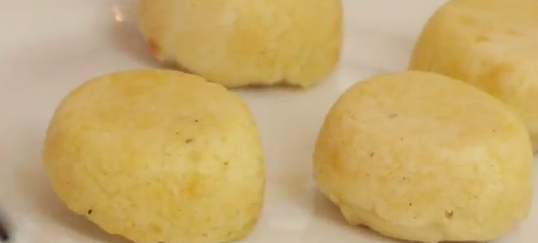
\includegraphics[scale=0.4]{IndianRiceCakes.png}
\end{center}


\end{document} 











